\section{Calibration using calibration gas}
\label{sec:no}

As a next step to characterize the \ch{NO}-measurement capabilities of
our modified CE-DOAS instrument, we conducted an experiment using
synthetic air and \ch{NO} calibration gas. Thus our sample air
was completely \ch{NO2} free, thus eliminating the need to subtract
multiple data points to get the \ch{NO} value. Furthermore this
allowed us to minutely control the \ch{NO} concentration leading to
very precise correlation measurements.

Additionally we wanted to see the influence of different reaction path
lengths on the timeseries of the \ch{NO} concentration has. The
behaviour of our system  after a very steep change of flow was of
special interested. We used it as an indicator to find out whether the
\ch{NO} conversion to \ch{NO2} was completed within the reaction tube
or still took place in the cavity.

\subsection{Setup}
\label{sec:no-setup}

The general setup can be found in Figure~\ref{fig:no-setup}. The
synthetic air and \ch{NO} container were attached to a flow control
unit with which we were able to set the flow ratio and in doing so the
mixing ratio of the two gases. In order to change the setup of the
cavity as little as possible, we decided not to bypass the DOAS main
pump using the Helium bypass, but instead built a bypass infront of
the lab air input to free ourselves of the excess current from the
pressurized containers. The synthetic air flow $\Phi_\text{air}$ was
set to \SI{3}{\liter\per\minute} and the \ch{NO} flow $\Phi_{\ch{NO}}$
was varied between \num{0} and \SI{0.03}{\liter\per\minute}. The DOAS
pump worked at a flow $\Phi$ of \SI{2}{\liter\per\minute} and the
Ozone generator supplied \SI{0.03}{\liter\per\minute} of that.

We used ambient lab air together with an I0 cartridge for our trace
gas free spectra and to for our Ozone generator.

\begin{figure}[htbp]
  \centering
  
\includegraphics[width=0.6\textwidth]{no_setup.png}
  \caption{Setup of the calibration measurement}
  \label{fig:no-setup}
\end{figure}

To later be able to compare the measured \ch{NO} concentration we have
to convert the applied \ch{NO} flow to a concentration, too. We can
do this using the following formula
\begin{align*}
  c_{\ch{NO}} = c_{\text{cont}} \cdot \frac{\Phi_{\ch{NO}}}{\Phi_{\text{air}} + \Phi_{\ch{NO}}}
\end{align*}

with the concentration $c_{\text{cont}}$ in the \ch{NO} container
given to be \SI{8.177}{ppb}. 

\subsection{Measurement results}
\label{sec:no-result}

Figure~\ref{fig:ts} Shows the timeseries of the \ch{NO} and \ch{O3}
concentration. Each of the three clusters corresponds from left to
right to the reaction path length of \num{5}, \num{10} and
\SI{15}{\meter}. The Ozone concentration is within the margin of its
error constant while we see that the overall shape of the \ch{NO}
timeseries does not depend on the pathlength. One deviation can be
found in the $l = \SI{5}{\meter}$ plot, where all the upward flanks
have a very long decay time before they reach the stable plateau.

\begin{figure}[htbp]
  \centering
  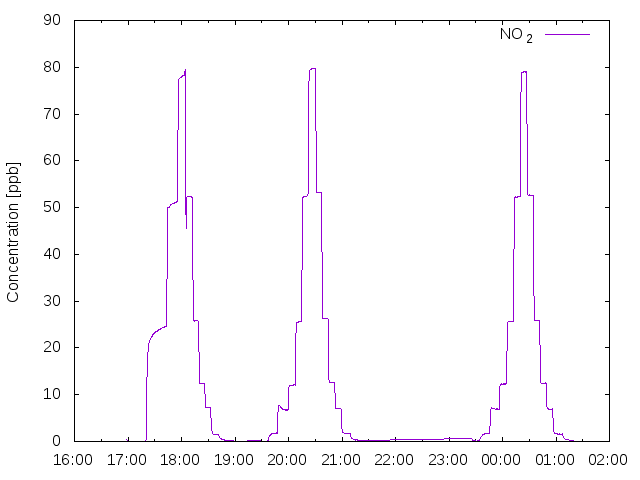
\includegraphics[width=0.45\textwidth]{20160222_NO_fixI0_NO_ts.png}
  \hfill
  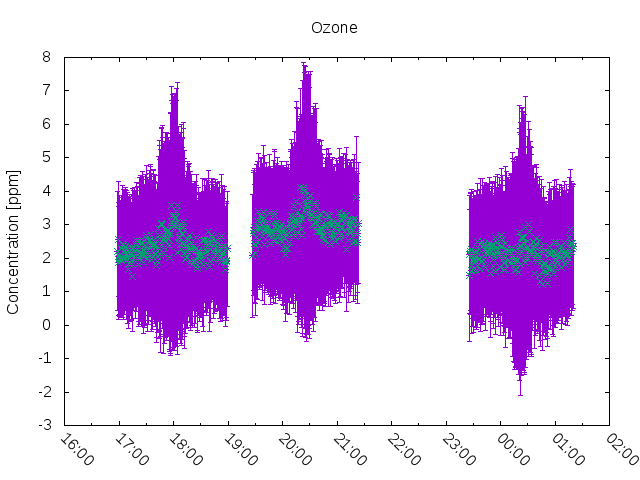
\includegraphics[width=0.45\textwidth]{20160222_NO_fixI0_O3_ts.png}
  \caption{Timeseries of the \ch{NO} and \ch{O3} concentration. The
    three clusters correspond to the three used reaction path lengths
    $l = 5, 10$ and \SI{15}{\meter}.}
  \label{fig:ts}
\end{figure}
\todo{Redo figures with sensible dimensions}

Averaging over regions of constant flow and plotting over the reaction
path length, we yield Figure~\ref{fig:no-length}. The figure also
contains linear interpolation of the data points. The plots together
with the fits imply that the measured \ch{NO} concentration does not
depend on the pathlength, as is well expected.

\begin{figure}[htbp]
  \centering
  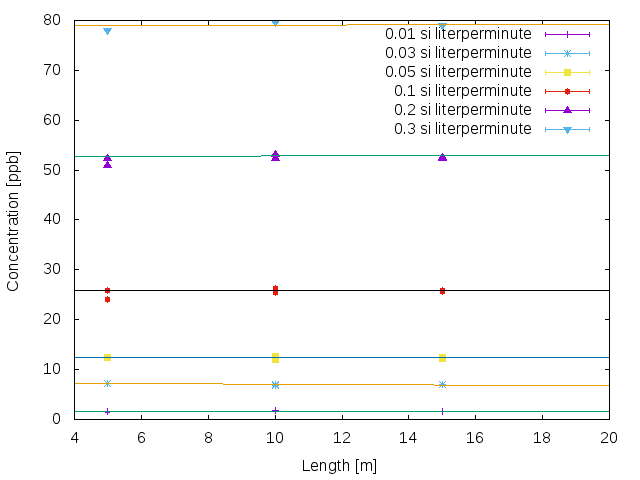
\includegraphics[width=0.75\textwidth]{20160222_NO_fixI0_NO_length.png}
  \caption{\ch{NO} concentration dependence on reaction path
    length. The data points are colored depending on the applied
    \ch{NO} flow. All data points were linearly interpolated. The
    results can also be found in the plot.}
  \label{fig:no-length}
\end{figure}

Since all measured concentration are pathlength independent, we can
all use them to compare the measured \ch{NO} concentration to the
computed \ch{NO} concentration. The summary is shown in
Figure~\ref{fig:no-calib}. The linear regression line follows the formula

\begin{align*}
  y = 0.994 \cdot x -0.00234.
\end{align*}

This is an exceptional accordance between the measured and the
computed mixing ratios.

\begin{figure}[htbp]
  \centering
  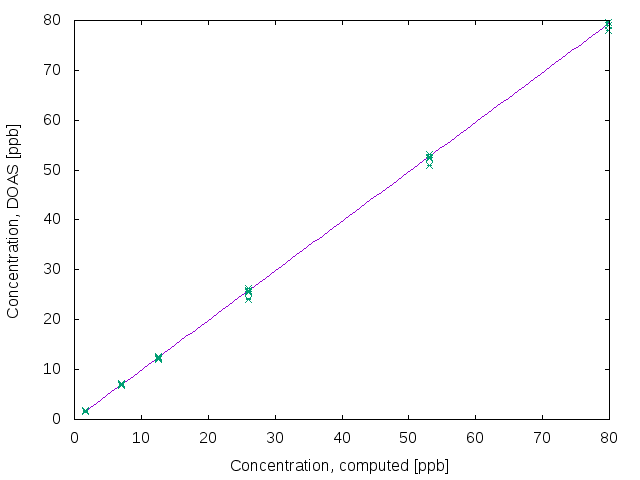
\includegraphics[width=0.75\textwidth]{20160222_NO_fixI0.png}
  \caption{Correlation plot of the computed and the measured \ch{pNO}
    concentration.}
  \label{fig:no-calib}
\end{figure}

%%% Local Variables:
%%% mode: latex
%%% TeX-master: "../Bachelor"
%%% End:
